\chapter{Functions and Their Graphs}

Functions are a major part of science, engineering, and math. You can think of a function as a machine: you put something into the
machine, it processes it, and out comes something else: a product. Just as we
often use the variable $x$ to stand in for a number, we often use the
variable $f$ to stand in for a function. $f(x)$ is said as ``f of x``.
% One of my teachers told me half of understanding math is understanding mathmaticions are just lazy, maybe a good add in somewhere

For example, we might ask, ``Let the function $f$ be defined like this:

\begin{equation*}
f(x) = -5x^2 + 12x + 2
\end{equation*}

What is the value of $f(3)$, said as ``f of 3``?

You would run the number 3 through ``the machine'': $-5(3^2) + 12(3) + 2 = -7$. The answer would be ``$f(3)$ is $7$''.

However, some functions are not defined for every possible input. For example:

\begin{equation*}
  f(x) = \frac{1}{x}
\end{equation*}

  This is defined for any $x$ except 0, because you can't divide 1 by 0. The set of values that a function can process is called its \textit{domain}, and resulting output values are called the range.
  It is important to note that functions have only one \emph{output} for each \emph{input}. However, multiple inputs can have the same output. 
  A relationship where one input can result in the more than one output is not a function, but a relation. This can be proven by the \hyperref[sec:vertical]{vertical line test}.
% some good images could be found here: https://www.ck12.org/book/ck-12-algebra-i-honors/section/3.1/ 

\begin{Exercise}[title={Domain of a function}, label=function_domain]

  Let the function $f$ be given by $f(x) = \sqrt{x - 3}$.  What is its domain?

\end{Exercise}
\begin{Answer}[ref=function_domain]
  You can only take the square root of nonnegative numbers, so the
  function is only defined when $x - 3 \geq 0$.  Thus, the domain is
  all real numbers greater than or equal to 3.
\end{Answer}

\section{Graphs of Functions}

If you have a function, $f$, its graph is the set of pairs $(x, y)$
such that $y = f(x)$.  We usually draw a picture of this set, called a \textit{graph}. 
The graph not only includes the picture, but also the values of x and y used to create it.

Here is the graph of the function $f(x) = -5x^2 + 12x + 2$:

\begin{tikzpicture}
    \begin{axis}[
        xmin=-1,xmax=3.5,
        ymin=-10,ymax=11,
        axis x line=middle,
        axis y line=middle,
        axis line style=<->,
        xlabel={$x$},
        ylabel={$y$},
        ]
        \addplot[no marks,sdkblue,<->] expression[domain=-0.7:3.05,samples=100]{(-5)*(x^2) + (12 * x) + 2}; 
    \end{axis}
\end{tikzpicture}

(Note that this is just part of the graph; it goes infinitely in both
directions. Remember your vectors!)

Here is the graph of the function $f(x) = \frac{1}{x}$:

\begin{tikzpicture}
    \begin{axis}[
        xmin=-7,xmax=7,
        ymin=-7,ymax=7,
        axis x line=middle,
        axis y line=middle,
        axis line style=<->,
        xlabel={$x$},
        ylabel={$y$},
        ]
        \addplot[no marks,sdkblue,<->] expression[domain=-6.5:-0.15,samples=100]{1/x}; 
        \addplot[no marks,sdkblue,<->] expression[domain=0.15:6.5,samples=100]{1/x}; 
    \end{axis}
\end{tikzpicture}
To draw a graph, take each x value (usually in increments of 1) and determine its corresponding y value. 
Then, plot those points on a graph, using the origin as the starting point. 
% do we assume students know how to graph?
\begin{Exercise}[title={Draw a graph}, label=draw_graph]

  Let the function $f$ be given by $f(x) = -3x + 3$. Sketch its graph.
% More space needed in exercise box
\end{Exercise}
\begin{Answer}[ref=draw_graph]

  The graph of this function is a line, its slope is -3, and it intersects the y axis at $(0, 3)$.

\begin{tikzpicture}
    \begin{axis}[
        xmin=-1,xmax=3,
        ymin=-7,ymax=7,
        xtick={1},
        ytick={3},
        axis x line=middle,
        axis y line=middle,
        axis line style=<->,
        xlabel={$x$},
        ylabel={$y$},
        ]
        \addplot[no marks,sdkblue,<->] expression[domain=-0.75:2.74,samples=100]{-3 * x + 3}; 
    \end{axis}
\end{tikzpicture}
  
  
\end{Answer}


\section{Can this be expressed as a function?}
\label{sec:vertical}

Note that not all sets can be expressed as graphs of functions.  For
example, here is the set of points $(x,y)$ such that $x^2 + y^2 = 9$:

\begin{tikzpicture}
    \begin{axis}[
        xmin=-3.5,xmax=3.5,
        ymin=-3.5,ymax=3.5,
        ytick={-3,-2,-1,0,1,2,3},
        axis x line=middle,
        axis y line=middle,
        axis line style=<->,
        xlabel={$x$},
        ylabel={$y$},
        ]
        \addplot[no marks,sdkblue] expression[domain=-3:3,samples=100]{sqrt(9 - x^2)}; 
        \addplot[no marks,sdkblue] expression[domain=-3:3,samples=100]{-1 * sqrt(9 - x^2)}; 
    \end{axis}
\end{tikzpicture}

This cannot be the graph of a function, because what would $f(0)$ be? 3
or -3?  This set fails what we call ``the vertical line test'': If any
vertical line contains more than one point from the set, it isn't the graph
of a function.  For example, the vertical line $x = 2$ would cross the graph twice:
\begin{center}
  
  \begin{tikzpicture}
    \begin{axis}[
      xmin=-3.5,xmax=3.5,
      ymin=-3.5,ymax=3.5,
      ytick={-3,-2,-1,0,1,2,3},
      axis x line=middle,
      axis y line=middle,
      axis line style=<->,
      xlabel={$x$},
      ylabel={$y$},
      ]
      \addplot[no marks,sdkblue] expression[domain=-3:3,samples=100]{sqrt(9 - x^2)}; 
      \addplot[no marks,sdkblue] expression[domain=-3:3,samples=100]{-1 * sqrt(9 - x^2)};
      \addplot [thick, dashed] coordinates {(2,-2.5)(2,2.5)};
      
    \end{axis}
    
  \end{tikzpicture}
\end{center}
%might be a good place to talk about even vs odd functions
\index{vertical line test}

\section{Inverses}

Some functions have inverse functions. If a function $f$ is a machine that turns
number $x$ into $y$, the inverse (usually denoted $f^{-1}$) is the machine that turns $y$ back
into $x$.

For example, let $f(x) = 5x + 1$. Its inverse is
$f^{-1}(x) = (x - 1)/5$. (Spot check it: $f(3) = 16$ and $f^{-1}(16) = 3$)

Does the function $f(x) = x^3$ have an inverse? Yes, $f^{-1}(x) =
\sqrt[3]{x}$. Let's plot the function (solid line) and its inverse (dashed):

\begin{tikzpicture}
    \begin{axis}[
        xmin=-3.5,xmax=3.5,
        ymin=-3.5,ymax=3.5,
        ytick={-3,-2,-1,0,1,2,3},
        axis x line=middle,
        axis y line=middle,
        axis line style=<->,
        xlabel={$x$},
        ylabel={$y$},
        ]
        \addplot[no marks,sdkblue] expression[domain=-3:3,samples=100]{x^3}; 
        \addplot[no marks,sdkblue,dashed] expression[domain=0:3,samples=100]{x^(1/3)}; 
        \addplot[no marks,sdkblue,dashed] expression[domain=-3:0,samples=100]{-1 * (-1 * x)^(1/3)}; 
    \end{axis}
\end{tikzpicture}

The inverse is the same as the function, just with its axes swapped.
The inverse function is \emph{reflected} across the line $y=x$. \index{reflections}
This tells us how to solve for an inverse: We swap $x$ and $y$ and
solve for $y$.

For example, if you are given the function $f(x) = 5x + 1$, its graph
is all $(x,y)$ such that $y = 5x + 1$.  The graph of its inverse is
all $(x, y)$, such that $x = 5y + 1$. Solving for $y$ gives you $y = (x -
1)/5$. So we can say that $f^{-1}(x) = (x - 1)/5$, QED.

Not every function has an inverse.  For example, $f(x) = x^2$.  Note
that $f(2) = f(-2) = 4$.  What would $f^{-1}(4)$ be? 2 or -2?  This
implies the ``horizontal line test'': If any horizontal line contains
more than one point of a function's graph, that function has no
inverse. If a function passes the horizontal line test, it is called 
"one-to-one", meaning there is exactly one $x$ that gives each $y$. \\
\index{horizontal line test}
\begin{center}
  \begin{tikzpicture}
    \begin{axis}[
      xmin=-3.5,xmax=3.5,
      ymin=-1, ymax=6,
      ytick={-1,0,1,2,3,4,5,6},
      axis x line=middle,
      axis y line=middle,
      axis line style=<->,
      xlabel={$x$},
      ylabel={$y$},
      ]
      \addplot[no marks,sdkblue] expression[domain=-3:3,samples=100]{x^2};
      \addplot [thick, dashed] coordinates {(-3,4)(3,4)};
    \end{axis}
  \end{tikzpicture}
\end{center}

In some problems, you need an inverse, but you don't need the
whole domain, so you trim the domain to a set you can define an
inverse on. This allow you to make claims such as ``If we restrict the domain to
the nonnegative numbers, the function $f(x) = x^2 - 5$ has an inverse:
$f^{-1}(x) =\sqrt{x + 5}$.

This raises the question: What is the domain of the inverse function $f^{-1}$?

If we let $X$ be the domain of $f$, we can run every member of $X$
through ``the machine'' and gather them in a set on the other
side. This set would be the \textit{image} of the $f$ "machine". (This is the \textit{range} of $f$.)

What is the image of $f(x) = x^2 - 5$? It is the set of all real
numbers greater than or equal to -5. We write this:

\begin{equation*}
  \{ x \in {\rm I\!R} | x \geq -5 \}
  \end{equation*}

Now we can say: \textbf{The range (or image) of the function is the domain
  of the inverse function.}

In inverse functions, the domain and range get swapped: 
the domain of the function is the range of the inverse function, and visa versa.
In our example, we can use any number greater
than or equal to -5 as input into the inverse function.

\begin{tikzpicture}
    \begin{axis}[
        xmin=-5.5,xmax=7.5,
        ymin=-6, ymax=5,
        xtick={-3, 2},
        ytick={-5, 1},
        axis x line=middle,
        axis y line=middle,
        axis line style=<->,
        ]
      \addplot[no marks,sdkblue, ->] expression[domain=0:3,samples=100]{x^2 - 5} node[right] {$y = x^2 - 5$};
      \addplot [thick, dashed, red, ->] coordinates {(-0.05,-5)(-0.05,4.5)}
      node [draw, red, left, align=left, yshift=-0.6cm, xshift=-0.1cm] {image of $f$ \textit{or}\\ domain of $f^{-1}$};
      \addplot [thick, dashed, blue, ->] coordinates {(-0,-5.1)(6.75,-5.1)}
      node [draw, align=left, above, blue, yshift=0.1cm, xshift=-1.3cm] {domain of $f$ \textit{or}\\image of $f^{-1}$};
    \end{axis}
\end{tikzpicture}


\begin{Exercise}[title={Find the inverse}, label=simple_inverse]

  Let $f(x) = (x - 3)^2 + 2$.  Sketch the graph.

  Using all the real numbers as a domain, does this function have an inverse?

  How would you restrict the domain to make the function invertible?

  What is the inverse of that restricted function?

  What is the domain of the inverse?

\end{Exercise}
\begin{Answer}[ref=simple_inverse]

  This graph is the graph of $y = x^2$ that has been moved to the right by three units and up two units:
 
\begin{tikzpicture}
    \begin{axis}[
        xmin=-1,xmax=7,
        ymin=-1,ymax=7,
        xtick={3, 6},
        ytick={2, 4},
        axis x line=middle,
        axis y line=middle,
        axis line style=<->,
        xlabel={$x$},
        ylabel={$y$},
        ]
      \addplot[no marks,sdkblue,<->] expression[domain=-2.5:6.5,samples=100]{(x - 3)^2 + 2};
      \addplot[dashed] coordinates {(-1, 2)(4,2)};
      \addplot[dashed] coordinates {(3, -1)(3, 3)};
    \end{axis}
\end{tikzpicture}

To prevent any horizontal line from containing more than one point of
the graph, you would need to use the left or the right side --- either
$\{x \in {\rm I\!R}  | x \leq 3\}$ or $\{x {\rm I\!R}| x \geq 3\}$. Most people will choose the
right side; the rest of the solution will assume that you did too.

To find the inverse we swap $x$ and $y$: $x = (y -3)^2 + 2$

Next, we solve for $y$ to get the inverse: $y = \sqrt{x - 2} + 3$

You can take the square root of nonnegative numbers. So the function
$f^{-1}(x) = \sqrt{x - 2} + 3$ is defined whenever $x$ is greater than
or equal to 2.

\end{Answer}

\begin{Exercise}[label=invfunc1]
A function is given by a table of values, a graph, or a written description. 
Determine whether it is one-to-one. 
	\begin{enumerate}
	\item
	\begin{tabular}{|c|c|c|c|c|c|c|}\hline
	$x$ & 1 & 2 & 3 & 4 & 5 & 6\\
	\hline
	$f(x)$ & 1.5 & 2.0 & 3.6 & 5.3 & 2.8 & 2.0\\
	\hline	
	\end{tabular}
	\item
	\begin{tabular}{|c|c|c|c|c|c|c|}\hline
	$x$ & 1 & 2 & 3 & 4 & 5 & 6\\
	\hline
	$f(x)$ & 1.0 & 1.9 & 2.8 & 3.5 & 3.1 & 2.9\\
	\hline	
	\end{tabular}
	\item
	\begin{tikzpicture}[scale=0.5]
		\begin{axis}
		[xmin=-2, xmax=2, xlabel=$x$,
		ymin=-0.5, ymax=4, ylabel=$y$,
		axis lines = center, ticks=none]
		\addplot[blue, thick, samples=100]{e^(-1*x^2)+1};
		\end{axis}
	\end{tikzpicture}
	\item
	\begin{tikzpicture}[scale=0.5]
		\begin{axis}
		[xmin=-1, xmax=3, xlabel=$x$,
		ymin=-2, ymax=2, ylabel=$y$,
		axis lines = center, ticks=none]
		\addplot[blue, thick, samples=100]{-ln(x+1)};
		\end{axis}
	\end{tikzpicture}
	\item $f(t)$ is the height of a football $t$ seconds after kickoff
	\item $v(t)$ is the velocity of a dropped object
	\end{enumerate}
\end{Exercise}

\begin{Answer}[ref=invfunc1]
	\begin{enumerate}
	\item This function is not one-to-one. From $x=3$ to $x=4$, the 
	function increases from 3.6 to 5.3, which means it must pass through 
	$f(x_1)=4.0$. From $x=4$ to $x=5$, the function decreases from 5.3 to 
	2.8, which means it must pass through $f(x_2) = 4.0$ again. 
	\item This function is not one-to-one by a similar argument in the 
	above solution
	\item This function is not one-to-one, because it fails the horizontal 
	line test
	\item This function is one-to-one, because it passes the horizontal 
	line test
	\item $f(t)$ would not be one-to-one because the football must pass 
	through each height (except the peak height) both on the way up and 
	on the way back down
	\item $v(t)$ would be one-to-one because a falling object only speeds 
	up. Therefore, every time has a unique speed. 
	\end{enumerate}
\end{Answer}

\section{Graphing Calculators}

One really easy way to understand your function better is to use a graphing
calculator. Desmos is a great, free online graphing calculator. 

In a web browser, go to Desmos: \url{https://www.desmos.com/calculator}

In the field on the left, enter the function $y = x^2 - x - 6$. (For
the exponent, just prefix it with a caret symbol: ``x\^{}2''.)

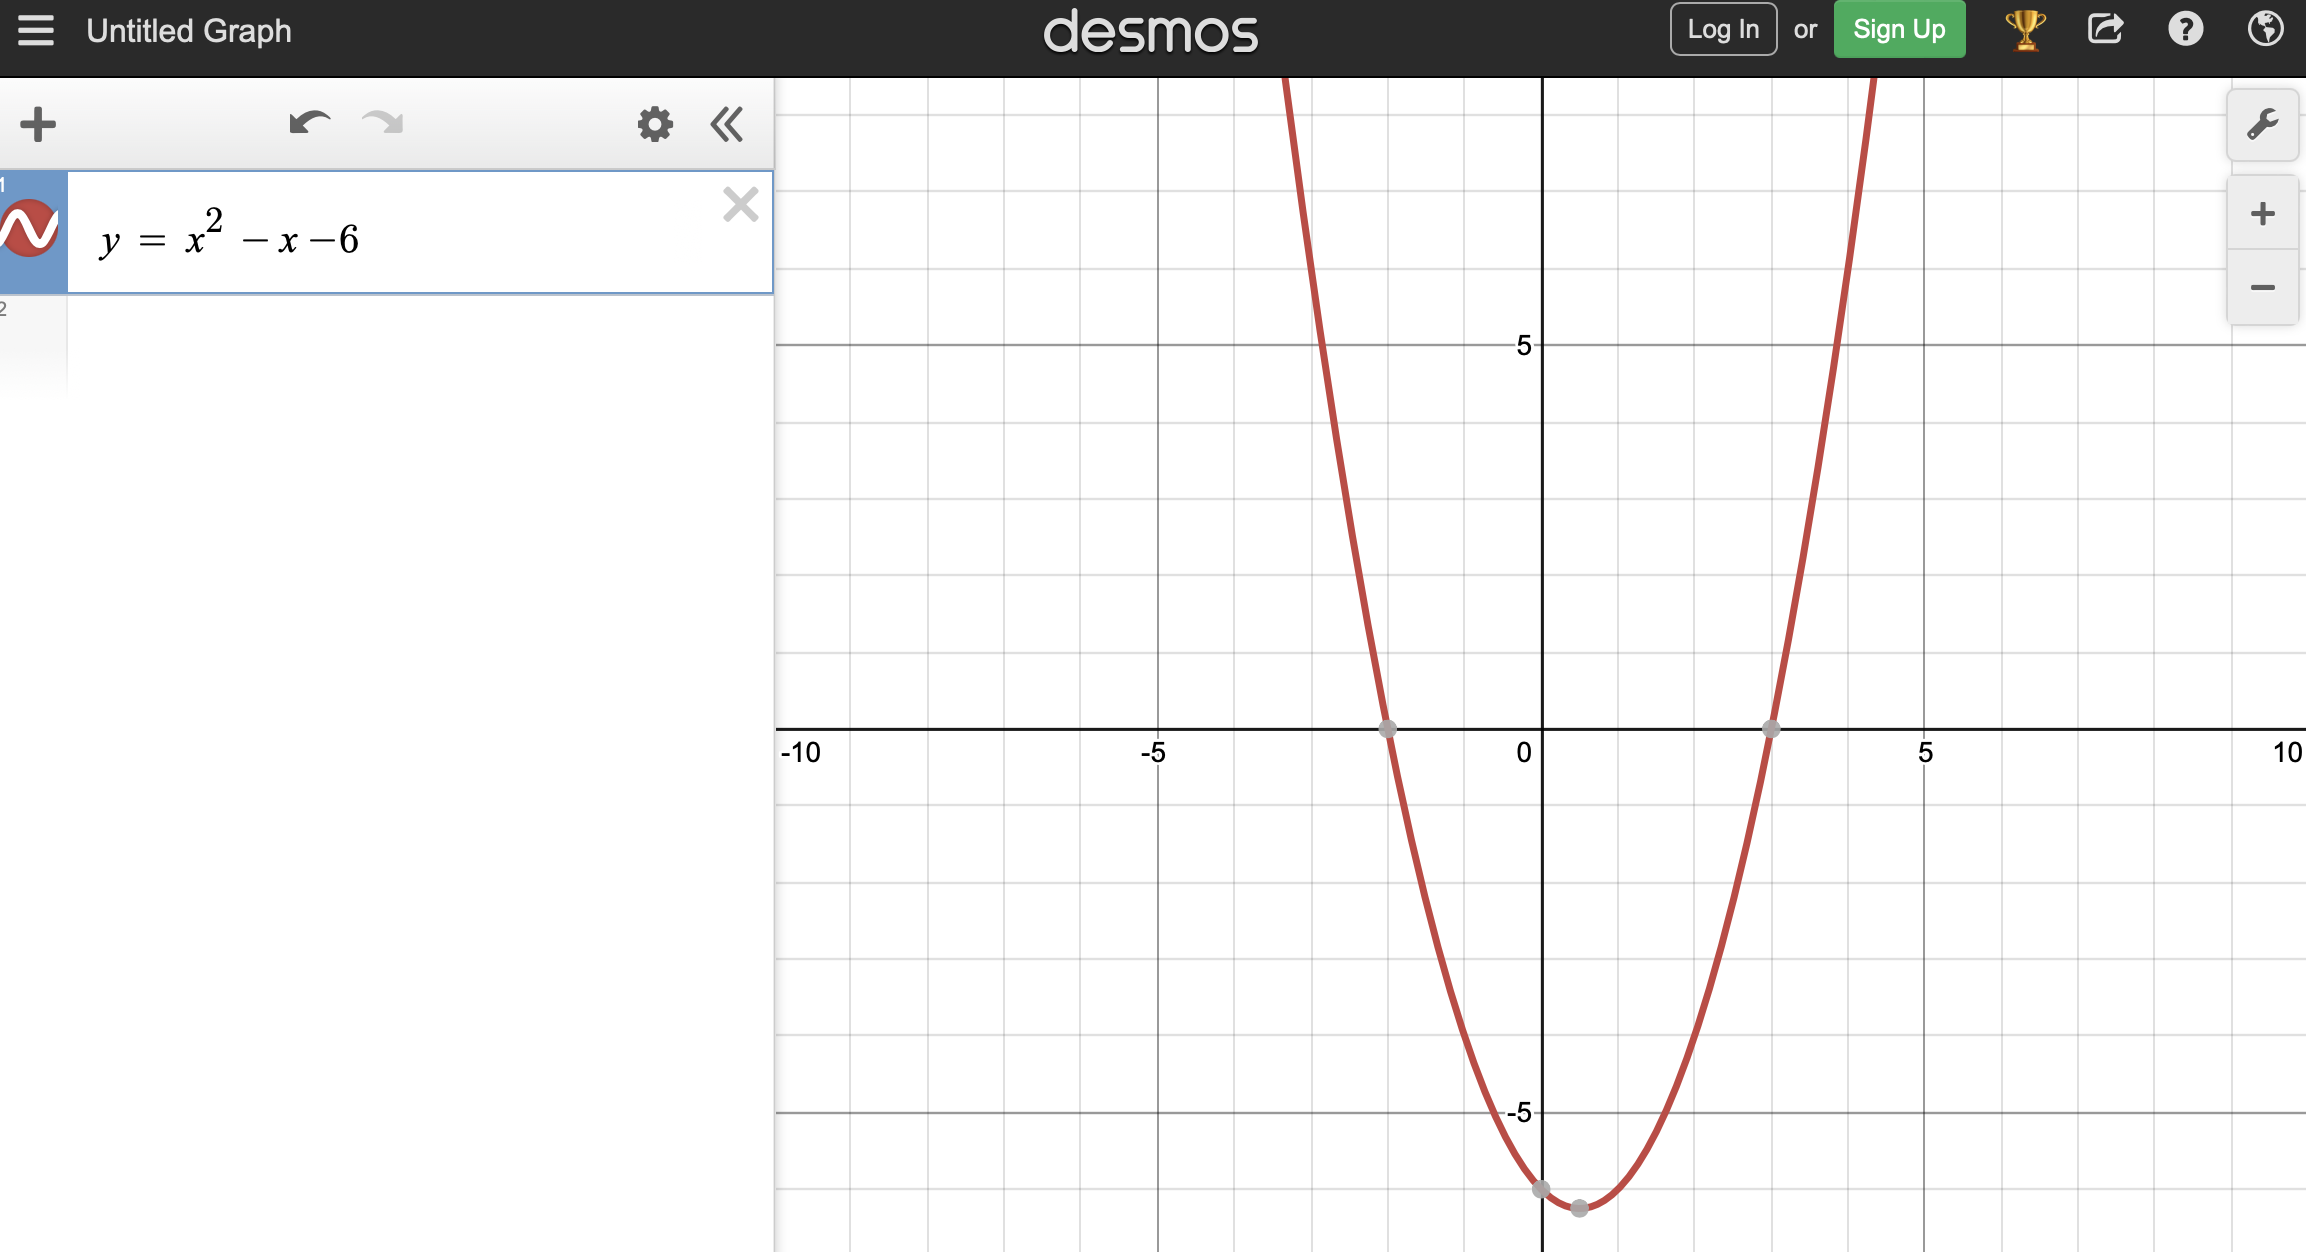
\includegraphics[width=0.85\textwidth]{Desmos.png}

\section{Even and Odd Functions}


\subsection{Even Functions}

An even function is symmetric about the y-axis. That means if you fold the graph along the y-axis, both sides will match perfectly. Note that the input value yields the same output regardless of whether the input value is positive or negative. 


\begin{mdframed}[style=important, frametitle={Even Functions}]

A function \( f(x) \) is even if  
\[
f(-x) = f(x)
\]  
for all \( x \) in its domain.
\end{mdframed}
Examples:
\begin{itemize}
  \item \( f(x) = x^2 \)  
  \item \( f(x) = \cos(x) \)  
  \item any \( f(x) = x^n \) where \( n \) is an even number
  \item \( f(x) = |x| \)
\end{itemize}

On a graph, a function will be a mirror image across the y-axis.

\subsection{Odd Functions}

An odd function is symmetric about the origin. That means if you rotate the graph $180^\circ$ about the origin, it lands on itself. Algebraically, when you input a value $k$, you get some output $n$; if you negate that input as $-k$, the output is also negated resulting in $-n$.


\begin{mdframed}[style=important, frametitle={Odd Functions}]

A function \( f(x) \) is odd if  
\[
f(-x) = -f(x)
\]
for all \( x \) in its domain.

Equivallently, 

\[ f(x) + f(-x) = 0 \]
for all \( x \) in its domain.
\end{mdframed}

\begin{itemize}

  \item \( f(x) = x^3 \)  
  \item \( f(x) = \sin(x) \)  
  \item \( f(x) = \tan(x) \)  
  \item any \( f(x) = x^n \) where \( n \) is an odd number
\end{itemize} 

On a graph, rotating the graph $180^\circ$ about the origin will yield the same graph.
\subsection{Neither Even Nor Odd}
Some functions are neither even nor odd. 

For example, \( f(x) = x^3 + 1 \) does not satisfy either condition.
% FIXME do we need to talk about end behavior, limits, symetry, etc